\chapter{Проектирование программного обеспечения}\label{ch:ch2}

\section{Проектирование визуального языка программирования}\label{sec:ch2/sec1}

Языку дано название \textbf{Flovver}.

Flovver --- аппликативный язык, то есть, вычислительный процесс в нем основывается на вычислении 
результата функции от заданного числа аргументов и передачи этого значения в другие функции.

На уровне семантики в языке существует всего-лишь один тип объектов --- функция.

Функция переводит от 0 до N значений заданных входящих типов в одно значение выходящего типа.

В Flovver функции представлены диаграммами вида, представленного на рисунке \ref{fig:functions}.

\begin{figure}[ht]
	\centering
	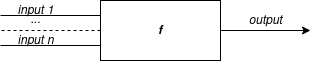
\includegraphics [scale=1.0] {functions}
	\caption{Представление функции в Flovver}
	\label{fig:functions}
\end{figure}
\FloatBarrier

Здесь блок $f$ --- некоторая функция типа $input~1$ $\rightarrow$ $\dots$ $\rightarrow$ $input~n$ $\rightarrow$ $output$. 
Левая часть блока --- входы функции, правая часть блока --- выход функции.

Из правой части выходит дуга, которую можно соединить с входом другой функции (рисунок \ref{fig:functions_composition}).

\begin{figure}[ht]
	\centering
	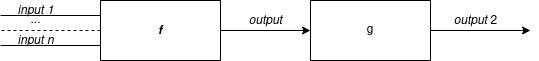
\includegraphics [scale=0.7] {functions_composition}
	\caption{Композиция функций в Flovver}
	\label{fig:functions_composition}
\end{figure}
\FloatBarrier

Если на вход переданы не все аргументы, считается, что функция недоопределена, и выходную дугу создать нельзя.

Функцию и переданные аргументы можно частично применить, проведя дугу из нижней стороны блока к месту использования (рисунок \ref{fig:thunks}).

\begin{figure}[ht]
	\centering
	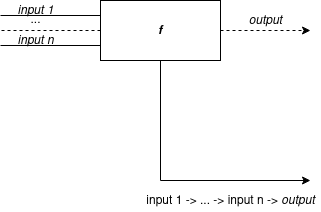
\includegraphics [scale=1.0] {thunks}
	\caption{Синтаксис частичного применения функции}
	\label{fig:thunks}
\end{figure}
\FloatBarrier

В результате получим из данной функцию от (нестрого) меньшего числа аргументов, ранее переданные аргументы будут зафиксированы (рисунок \ref{fig:thunks_example}).

\begin{figure}[ht]
	\centering
	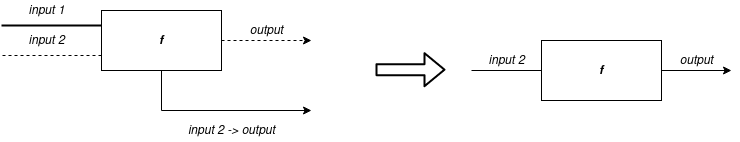
\includegraphics [scale=0.6] {thunks_example}
	\caption{Пример частичного применения функции}
	\label{fig:thunks_example}
\end{figure}
\FloatBarrier

Чтобы вычислить функцию, передаваемую как значение, можно использовать специальную функцию $apply$ (рисунок \ref{fig:apply_thunk}).

\begin{figure}[ht]
	\centering
	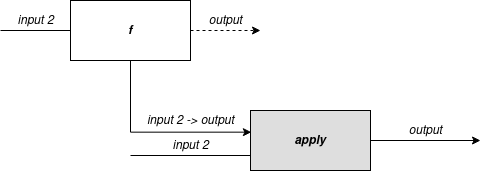
\includegraphics [scale=0.8] {apply_thunk}
	\caption{Пример использования специальной функции apply}
	\label{fig:apply_thunk}
\end{figure}
\FloatBarrier

Функция $apply$ принимает первым параметром функцию от N аргументов, следующие 2 ... N+1 параметров --- аргументы, подставляемые в первую функцию (рисунок \ref{fig:apply}).

\begin{figure}[ht]
	\centering
	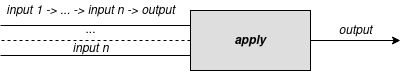
\includegraphics [scale=1.0] {apply}
	\caption{Синтаксис функции apply}
	\label{fig:apply}
\end{figure}
\FloatBarrier

Построение новых функций из заданных представлено на рисунке \ref{fig:function_body}.

\begin{figure}[ht]
	\centering
	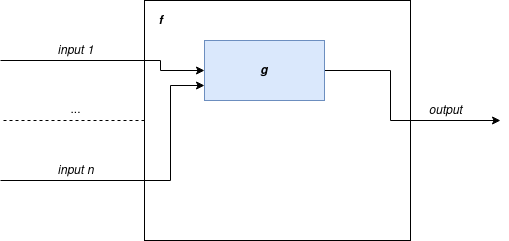
\includegraphics [scale=0.9] {function_body}
	\caption{Построение новой функции}
	\label{fig:function_body}
\end{figure}
\FloatBarrier

Здесь блок f --- тело функции, левая сторона блока --- входы функции, правая сторона блока --- выход функции; внутри блока находится функция $g$, к которой применяются входы $f$, результат $g$ передается на выход $f$.

Для поддержки создания рекурсивных функций внутри тела функции возможно создание специального блока $self$, который является ссылкой на объявляемую функцию (рисунок \ref{fig:function_body_self}).

\begin{figure}[ht]
	\centering
	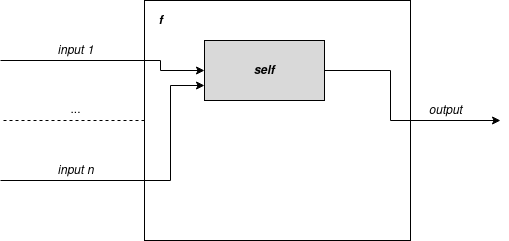
\includegraphics [scale=0.9] {function_body_self}
	\caption{Определение рекурсивной функции}
	\label{fig:function_body_self}
\end{figure}
\FloatBarrier

Можно считать, что функции с $self$ применены к комбинатору неподвижной точки. Комбинатором неподвижной точки (также Y-комбинатором) называют специальную функцию высшего порядка, которая вычисляет неподвижную точку другой функции \cite{tapl}. 
Практическая ценность такой функции --- возможность использовать рекурсию для анонимных функций без необходимости определения им имени.

Пример эквивалентной семантики, реализованной в языке Racket с использованием синтаксических макросов:

\begin{lstlisting}
;; Комбинатор неподвижной точки
(define Y
(lambda (f)
	((lambda (g) (g g))
	(lambda (g)       
		(f  (lambda a (apply (g g) a)))))))

;; Макрос, "эмулирующий" семантику self в Flovver.
(define-syntax-rule (combine self args f)
(Y (lambda (self) (lambda args f))))

;; Факториал, написанный с использованием self
(define fac
(combine self (x)
			(if (< x 2)
				1
				(* x (self (- x 1))))))

;; Функция Фибоначчи, написанная с использованием self
(define fib
(combine self (x)
			(if (< x 2)
				x
				(+ (self (- x 1)) (self (- x 2))))))

(fac 10)
(fib 5)  
\end{lstlisting}

\FloatBarrier

\section{Проектирование общей архитектуры приложения}\label{sec:ch2/sec2}

Рассмотрим общую архитектуру приложения, изображенную на рисунке \ref{fig:common_arch}.

Архитектура включает одно лицо --- пользователя (прикладного программиста),
и три компонента: компилятор, языковой сервер и среду разработки.

\begin{figure}[ht]
	\centering
	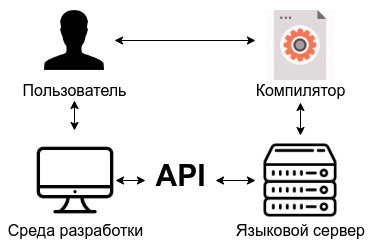
\includegraphics [scale=0.8] {common_arch}
	\caption{Общая архитектура разрабатываемого программного обеспечения}
	\label{fig:common_arch}
\end{figure}
\FloatBarrier

Пользователь имеет возможность формировать программы в интерактивном режиме
с помощью среды программирования, в том числе --- компилировать и запускать
получившееся приложение. Кроме этого, пользователь может собрать программу
из имеющихся данных вручную -- с помощью интерфейса командной строки
компилятора. Процесс работы пользователя с системой программирования во времени
показан на диаграмме последовательности на рисунке \ref{fig:arch-sequence}.

\begin{figure}[ht]
	\centering
	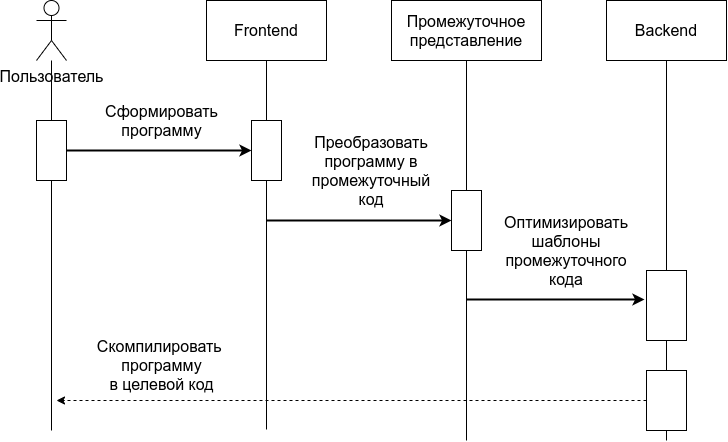
\includegraphics [scale=0.5] {arch-sequence}
	\caption{Диаграмма последовательности работы пользователя с системой}
	\label{fig:arch-sequence}
\end{figure}
\FloatBarrier

Из рисунка \ref{fig:common_arch} имеем зависимость между средой программирования
и компилятором. Зависимость не может быть прямой, так как компоненты системы
в общем случае не связаны между собой, и могут быть реализованы с использованием
совершенно разного набора технологий. Для связи среды и компилятора введен
компонент <<языковой сервер>>, являющийся шлюзом для сообщений, поступающих от
среды, и требующих выполнения в компиляторе. Было решено построить шлюз как
REST API, доступ к которому осуществляется по протоколу HTTP.

Интерфейс имеет следующие доступные по HTTP маршруты:

\begin{itemize}
	\item \textbf{/api/compile} (метод GET) --- вызывает сборку проекта в директории с работающим сервером;
	\item \textbf{/api/load} (метод GET) --- передает просящему конфигурацию проекта в формате JSON;
	\item \textbf{/api/save} (метод POST) --- сохраняет переданные в теле запроса данные в формате JSON как конфигурацию проекта.
\end{itemize}

Кроме вышеперечисленных, имеются маршруты общего назначения:
\begin{itemize}
	\item \textbf{/} (метод GET) --- корневой маршрут, по которому доступен сеанс работы в интегрированной среде;
	\item \textbf{/preview} (метод GET) --- маршрут, по которому доступна последняя собранная версия текущего проекта.
\end{itemize}

\section{Проектирование вариантов использования приложения}\label{sec:ch2/sec3}

Были написаны возможные сценарии действий пользователей.

\begin{enumerate}
    \item Тим-лид Иван побывал на стоячей встрече, откуда узнал, что его команда будет разрабатывать приложение <<Список задач>>.
	Иван хочет сделать прототип, чтобы объяснить задачу остальным членам команды.
    Он создает новый проект в приложении Flovver, описывает модель данных: текстовый список задач (нужно где-то хранить задачи). 
    Далее Иван начинает делать макет --- добавляет поле для ввода, кнопку и текстовый список.
    Иван сразу настроил макет, чтобы текст для списка брался из списка в модели данных.
    Теперь он хочет, чтобы при нажатии на кнопку текст из формы добавлялся в список. Он рисует простую программу на Flovver, которая это и делает.
    Иван включает прототип, смотрит, что все работает как надо, собирает программу и идет показывать другим членам команды.

    \item У программиста Олега ответственная задача --- ему надо добавить функцию <<Удаление элементов>> из списка в приложение <<Список задач>>.
	Олег открывает проект в Flovver и видит, что ему надо поменять только макет приложения и логику программы.
	В макете Олег добавляет элементам списка кнопку <<Удалить>> и идет менять логику программы. Олег добавляет функцию удаления в программу,
	запускает прототип, проверяет, что все работает и идет показывать результат другим членам команды.

    \item Дизайнеру Афанасию поручили подобрать цвет кнопки <<Добавить задачу>> вместе с заказчиком Михаилом.
	Афанасий открыл проект в Flovver и по желанию Михаила меняет цвет кнопки. Через пятнадцать минут Михаил
	определился с цветом кнопки и попросил выделить текст в кнопке курсивом, что Афанасий и сделал. Афанасий
	показал рабочий прототип Михаилу, обе стороны остались довольны резульататом.

    \item Аналитик Игорь решил, что в приложении <<Список задач>> кроме задачи нужно указывать также ориентировочную дату
	выполнения. Он открыл проект <<Список задач>> в Flovver, заменил модель данных <<Текстовый список задач>>
	на модель <<Список кортежей (Дата, Текст задачи)>>. Игорь попытался запустить прототип, но Flovver отказался запускать его,
	сообщив <<В программе не соответствуют типы данных --- ожидался Текстовый список задач, получили Список кортежей (Дата, Текст задачи)>>.
	К счастью, Игорь не запаниковал, отменил внесенные изменения и позвал программиста Олега.
	Олег выслушал Игоря, изменил модель и программу.
\end{enumerate}

\section{Проектирование интерфейса приложения}\label{sec:ch2/sec4}

\subsection{Проектирование меню и функционально-модульной структуры}\label{sec:ch2/sec4/subsec1}

При открытии программы должен появиться список настроек проекта. В верхней части рабочей области находится навигационное
меню с возможностью перехода в модули «Модель», «Обновление», «Представление», «Настройки». Также на верхней панели
находятся кнопки «Собрать» и «Запустить», при нажатии на которых происходит сборка проекта, запуск сборки проекта в отдельном окне соответственно.

\begin{figure}[ht]
	\centering
	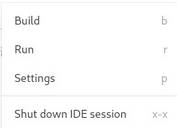
\includegraphics [scale=0.8] {dropdown}
	\caption{Компонент <<Выпадающее окно>>, появляющийся при нажатии на кнопку <<Проект>> на навигационной панели}
	\label{fig:dropdown}
\end{figure}
\FloatBarrier

В модуле «Настройки» содержится форма для управления флагами проекта: «Устранение хвостовой рекурсии»,
«Устранение рекурсии Фибоначчи», «Устранение общей рекурсии», которые представлены элементами управления
типа «Флаг» (англ. –-- check-box). Запись флагов в системное хранилище осуществляется при нажатии
на кнопку «Сохранить» в нижней части формы.

\begin{figure}[ht]
	\centering
	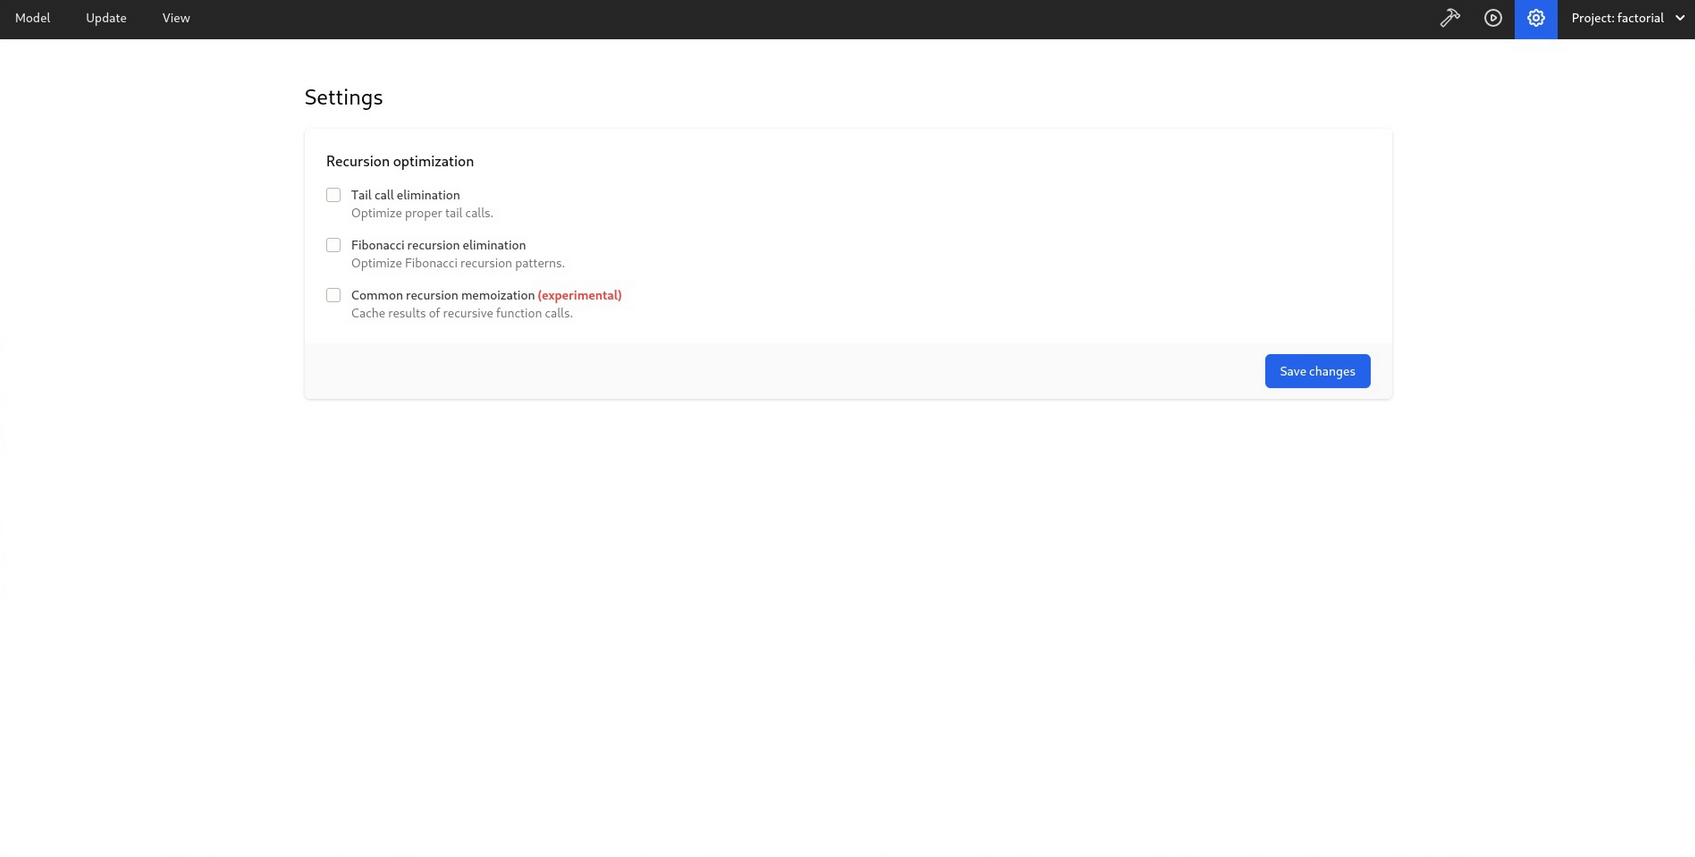
\includegraphics [scale=0.4] {settings_screen}
	\caption{Экран модуля <<Настройки>>, являющийся стартовым}
	\label{fig:settings_screen}
\end{figure}
\FloatBarrier

В модулях «Модель», «Представление», «Обновление» содержится рабочая область, представляющая пустое пространство,
на котором можно размещать элементы предметной области модуля используя механизм «drag-and-drop».

\begin{figure}[ht]
	\centering
	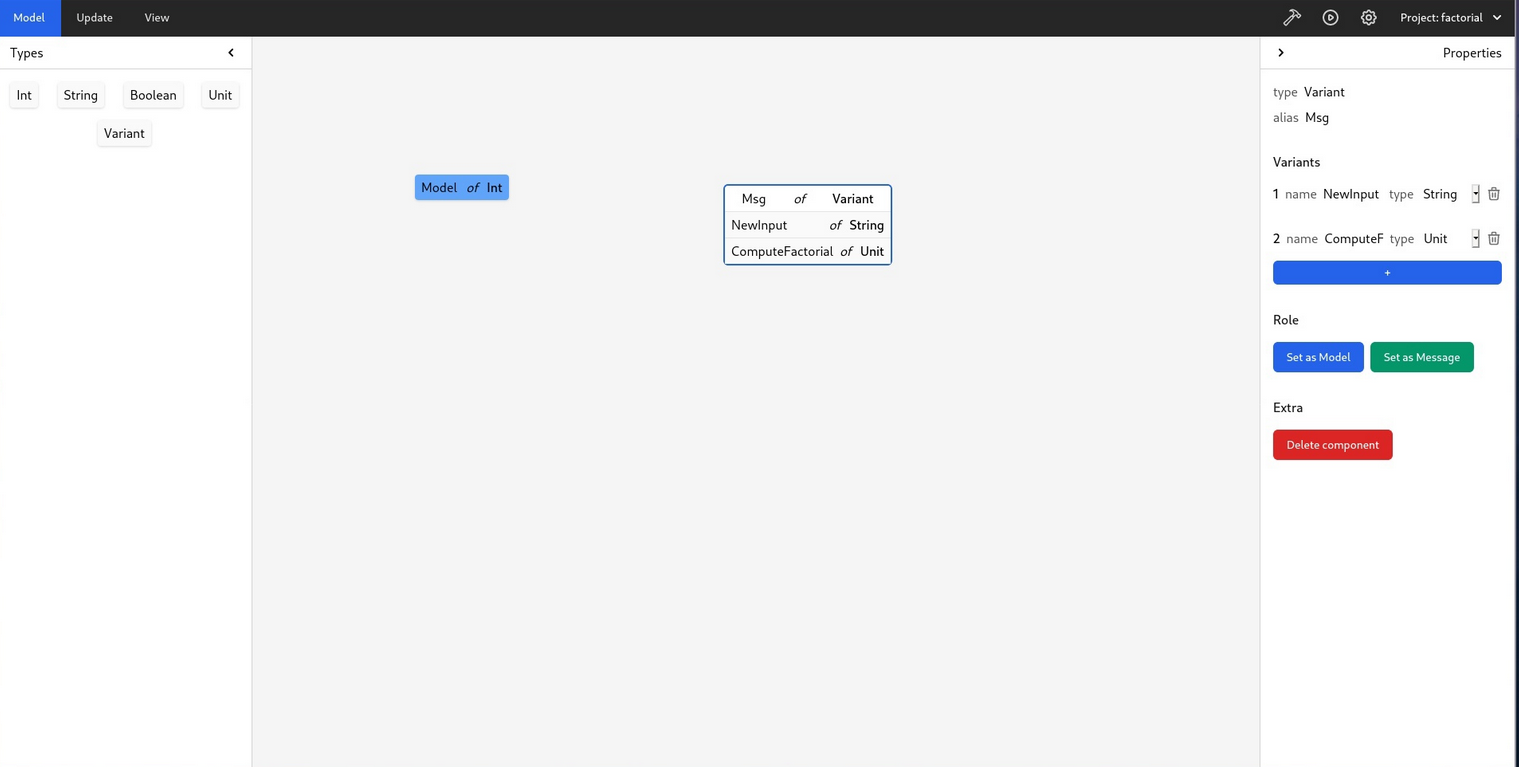
\includegraphics [scale=0.4] {model_screen}
	\caption{Экран модуля <<Модель>>}
	\label{fig:model_screen}
\end{figure}

\begin{figure}[ht]
	\centering
	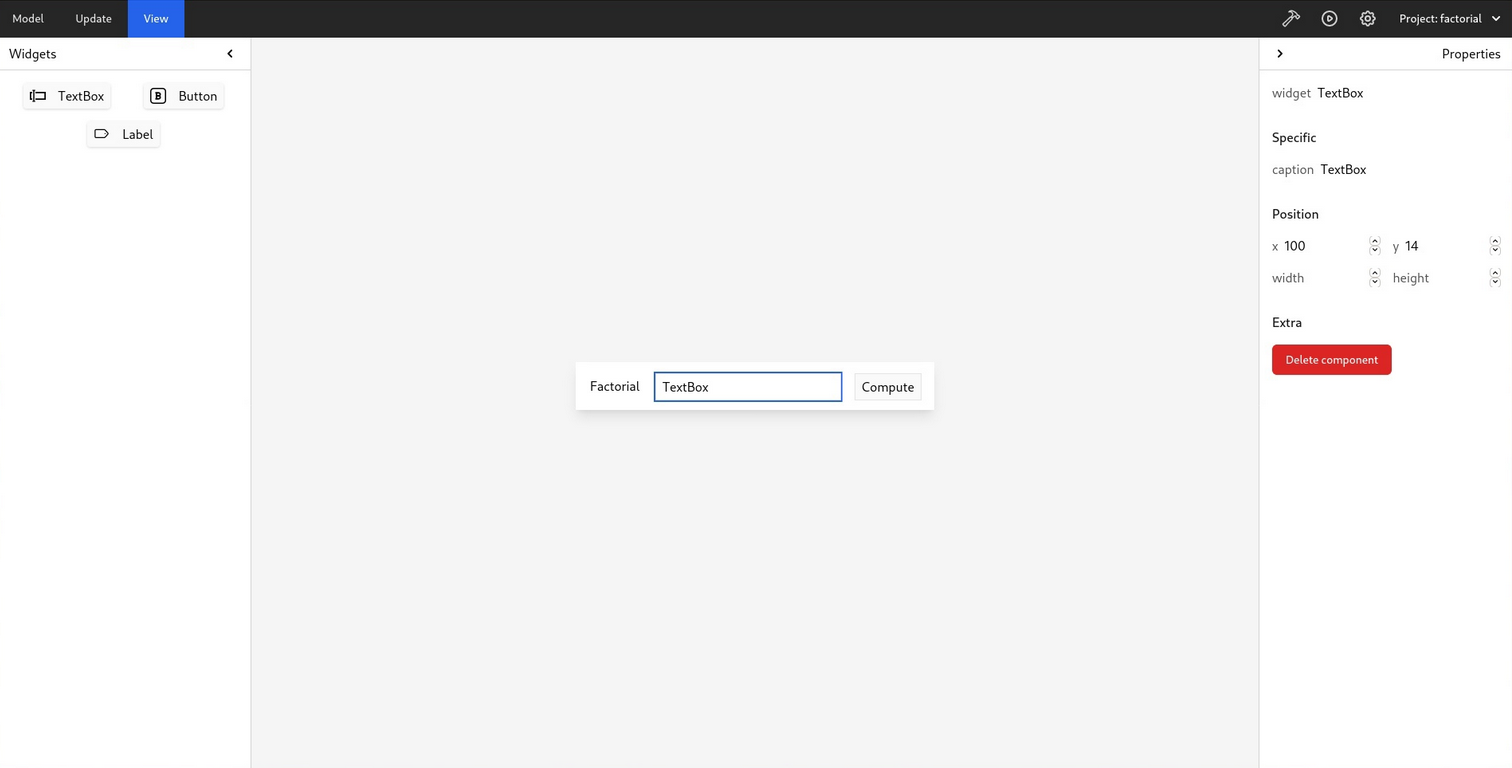
\includegraphics [scale=0.4] {view_screen}
	\caption{Экран модуля <<Представление>>}
	\label{fig:view_screen}
\end{figure}

\begin{figure}[ht]
	\centering
	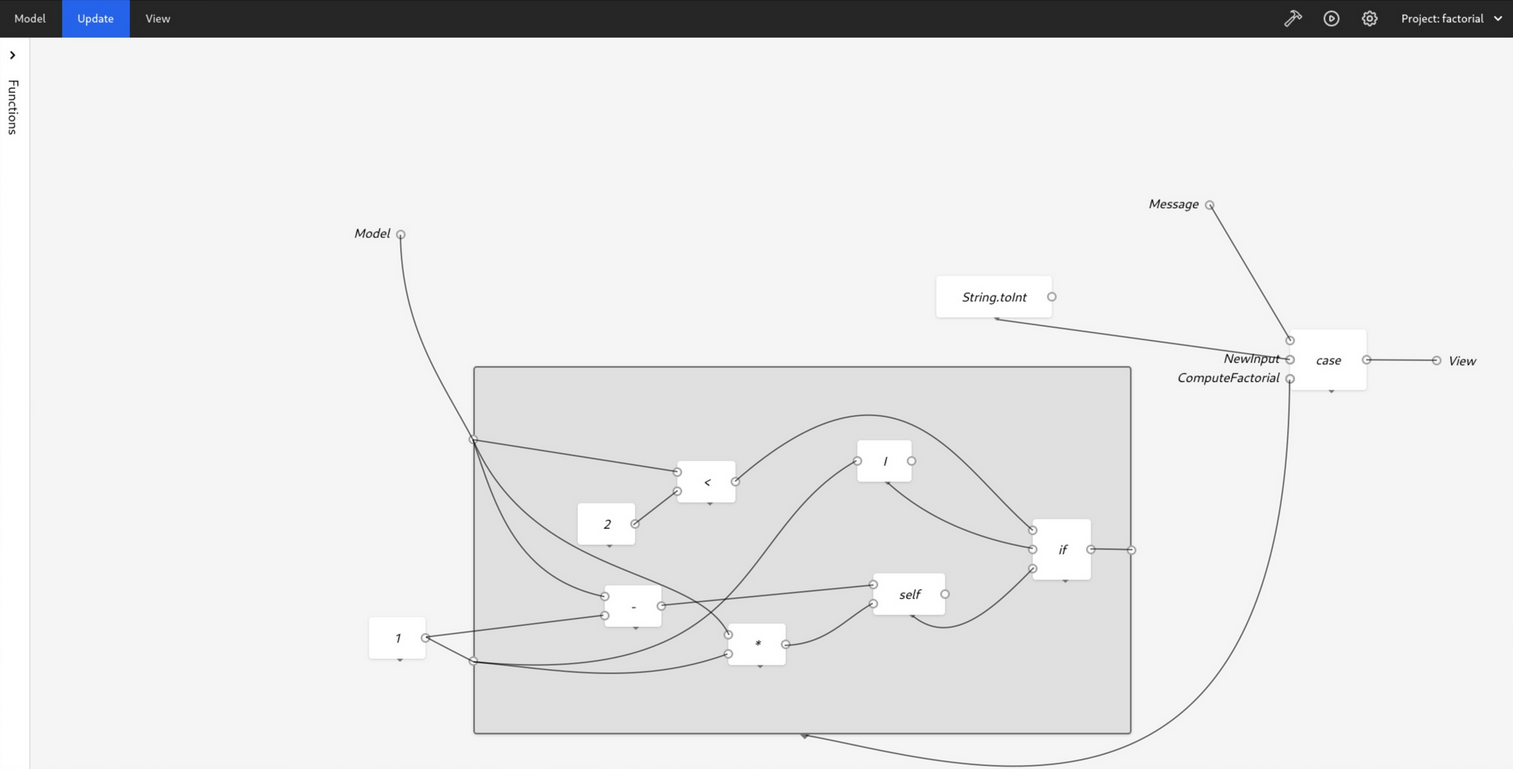
\includegraphics [scale=0.4] {update_screen}
	\caption{Экран модуля <<Обновление>>}
	\label{fig:update_screen}
\end{figure}

\FloatBarrier

Поверх рабочего окна в модулях находятся две боковые панели.
В левой части находится панель с сущностями предметной области модуля,
которые можно выбирать наведением и нажатием курсора,
добавлять в рабочую область перемещением курсора с зажатой левой кнопкой мыши.

\begin{figure}[ht]
	\centering
	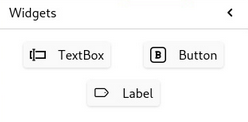
\includegraphics [scale=0.7] {widgets_panel}
	\caption{Левая боковая панель <<Виджеты>> модуля <<Представление>>}
	\label{fig:widgets_panel}
\end{figure}

\begin{figure}[ht]
	\centering
	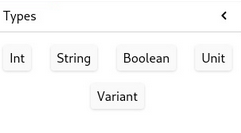
\includegraphics [scale=0.7] {model_types}
	\caption{Левая боковая панель <<Типы>> модуля <<Модель>>}
	\label{fig:model_types}
\end{figure}

\FloatBarrier

В правой части содержится панель свойств текущего объекта.
При нажатии левой кнопкой мыши на объект рабочей области,
для него отображается соответствующий набор свойств –-- имя объекта, его позиция и т.д.
Значения свойств изменяются с использованием соответствующих элементов управления --– форм ввода, кнопок.
При изменении объекта в рабочей области меняются значения его свойств на панели «Свойства» и наоборот.

\begin{figure}[ht]
	\centering
	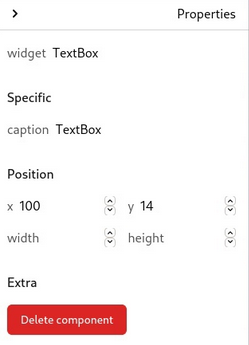
\includegraphics [scale=0.7] {view_properties}
	\caption{Правая боковая панель <<Свойства>> модуля <<Представление>>}
	\label{fig:view_properties}
\end{figure}

\begin{figure}[ht]
	\centering
	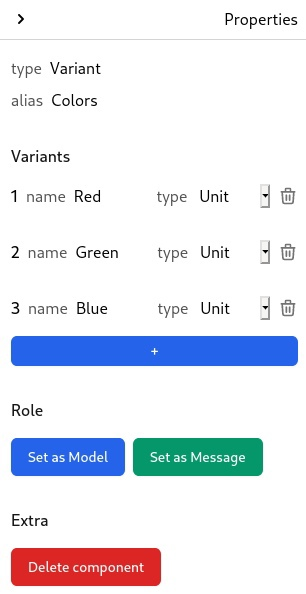
\includegraphics [scale=0.5] {model_properties}
	\caption{Правая боковая панель <<Свойства>> модуля <<Модель>>, выбран компонент <<Вариант>>}
	\label{fig:model_properties}
\end{figure}

\FloatBarrier

Панели можно сворачивать, нажимая на кнопку с соответствующим символом (иконки <<Стрелка влево>>, <<Стрелка вправо>>).

Объекты модуля «Модель» можно назначить моделью проекта. На панели «Свойства» содержится
раздел «Роли» с кнопкой «Назначить моделью». При нажатии на нее, выделенный объект помечается как модель.
В рабочем пространстве модель визуально представлена объектом с голубым фоном. Объекты типа «Вариант»
можно также назначить типом сообщений проекта. При фокусе на варианте в раздел «Роли» добавляется новая
кнопка «Назначить типом сообщений». Тип-сообщение выделяется в рабочем пространстве зеленой обводкой объекта.

\begin{figure}[ht]
	\centering
	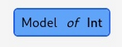
\includegraphics [scale=0.7] {model_model}
	\caption{Компонент <<Псевдоним примитивного типа>> модуля <<Модель>> в состоянии <<Назначен моделью>>}
	\label{fig:model_model}
\end{figure}

\begin{figure}[ht]
	\centering
	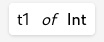
\includegraphics [scale=0.7] {model_primitive}
	\caption{Компонент <<Псевдоним примитивного типа>> модуля <<Модель>> в начальном состоянии}
	\label{fig:model_primitive}
\end{figure}

\begin{figure}[ht]
	\centering
	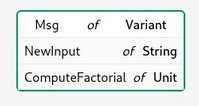
\includegraphics [scale=0.7] {message_variant}
	\caption{Компонент <<Тип-вариант>> модуля <<Модель>> в состоянии <<Назначен типом сообщений>>}
	\label{fig:message_variant}
\end{figure}

\begin{figure}[ht]
	\centering
	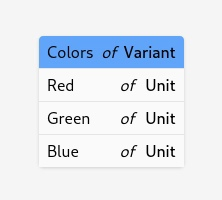
\includegraphics [scale=0.7] {model_variant}
	\caption{Компонент <<Тип-вариант>> в состоянии <<Назначен моделью>>}
	\label{fig:model_variant}
\end{figure}

\begin{figure}[ht]
	\centering
	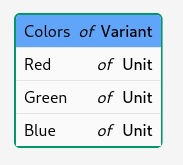
\includegraphics [scale=0.7] {message_model_variant}
	\caption{Компонент <<Тип-вариант>> в состоянии <<Назначен моделью и типом сообщений>>}
	\label{fig:message_model_variant}
\end{figure}

Объекты модуля «Обновление» можно соединять между собой связями. При нажатии
на выход одного объекта, появится черная линия, которую можно соединить с входом
другого объекта. При отжатии левой кнопки мыши вне входа функции, линия исчезнет
и связь не будет создана. Входы объекта <<Определение функции>> можно соединить
с входами лежащих в нем компонентов, также можно выходы объектов, лежащих внутри
компонента <<Определение функции>>, соединить с выходом этого объекта.
При соединении выхода какого-либо объекта с входом объекта, уже имеющего связь
по этому входу, прежняя связь удаляется, формируется последняя вызванная связь.

\begin{figure}[ht]
	\centering
	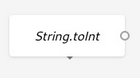
\includegraphics [scale=0.7] {update_call}
	\caption{Компонент <<Вызов функции>> модуля <<Обновление>>}
	\label{fig:update_call}
\end{figure}

\begin{figure}[ht]
	\centering
	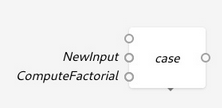
\includegraphics [scale=0.7] {update_case}
	\caption{Компонент <<Выбор варианта>> модуля <<Обновление>>}
	\label{fig:update_case}
\end{figure}

\begin{figure}[ht]
	\centering
	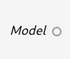
\includegraphics [scale=0.7] {update_input}
	\caption{Компонент <<Точка входа>> модуля <<Обновление>>}
	\label{fig:update_input}
\end{figure}

\begin{figure}[ht]
	\centering
	
\includegraphics [scale=0.7] {update_output}
	\caption{Компонент <<Точка выхода>> модуля «Обновление»}
	\label{fig:update_output}
\end{figure}

\begin{figure}[ht]
	\centering
	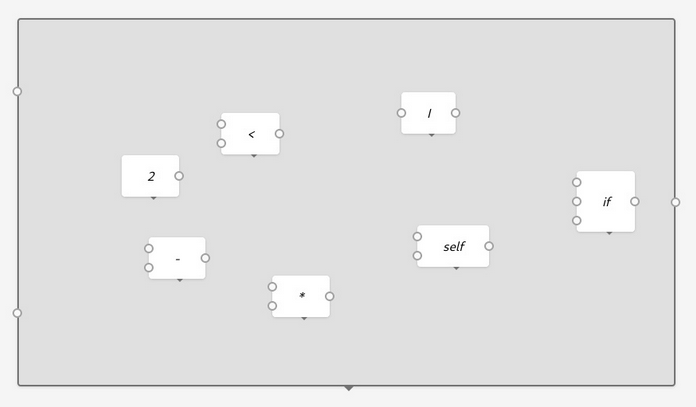
\includegraphics [scale=0.5] {update_def}
	\caption{Компонент <<Определение функции>> модуля <<Обновление>>}
	\label{fig:update_def}
\end{figure}

\begin{figure}[ht]
	\centering
	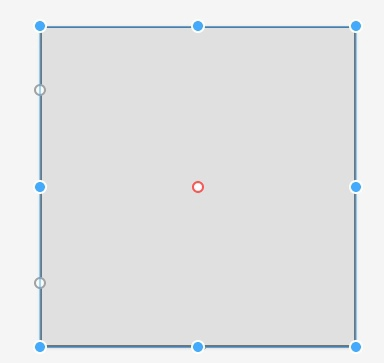
\includegraphics [scale=0.5] {update_def_band}
	\caption{Компонент <<Определение функции>> в состоянии <<Растягивание>>}
	\label{fig:update_def_band}
\end{figure}

\FloatBarrier

\newpage

\subsection{Полная функционально-модульная схема приложения}\label{sec:ch2/sec4/subsec3}

\begin{figure}[ht]
	\centering
	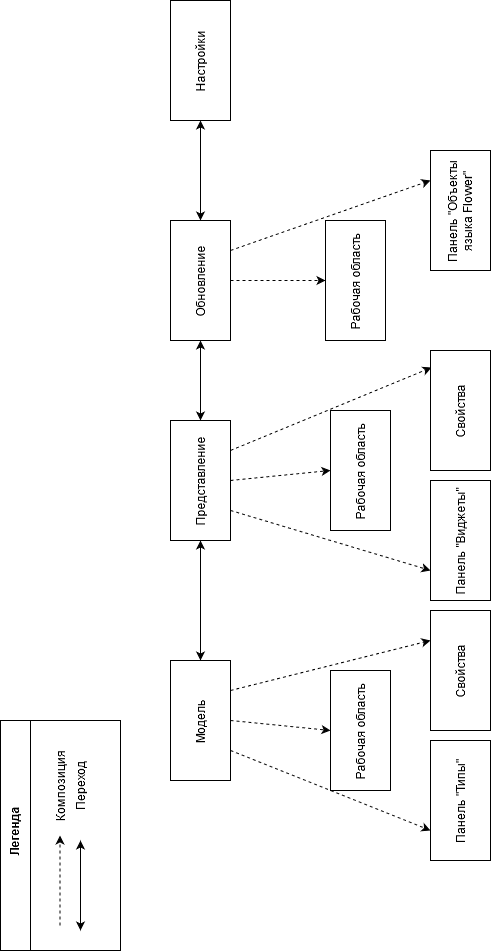
\includegraphics [scale=0.5] {full_scheme}
	\caption{Полная схема вкладок приложения}
	\label{fig:full_scheme}
\end{figure}

\FloatBarrier